\chapter{RIOT-OS and The GNRC Network Stack}
\section{RIOT Operating System}
  RIOT, the friendly operating system for the Internet of Things, is a real-time operating system,
  specifically designed for low-end IoT devices with a minimal memory in order of $\approx$ 10K Byte
  \cite{riot}. It can run on devices with neither memory management unit (MMU) nor memory protection unit (MPU).

  Under the distribution of LGPLv2.1 License, RIOT is free and open-source software, meaning it can
  be used and distributed by anyone. Furthermore, this license allows the linkage of RIOT with
  proprietary software and supports the ability to be customized by the end users.

  The design objectives of RIOT focus on several key areas: optimizing resource usage such as RAM, 
  ROM, and power consumption; supporting a broad spectrum of configurations, from 8-bit to 32-bit MCUs, 
  and accommodating various boards and use cases; reducing code duplication across different setups; 
  ensuring most of the code is portable across supported hardware; offering user-friendly software 
  platform; and enabling real-time capabilities. To realize these goals, one of the principles that
  the RIOT follows is modularity. 

  RIOT is organized into software modules that are combined at compile time, centered around a kernel 
  offering minimal functionality. This modular approach allows the system to be built in a way that includes 
  only the necessary modules for a given use case. As a result, both memory usage and system complexity 
  are kept to a minimum in practical deployments. The code structure of RIOT is illustrated in
  Figure \ref{fig:riot_code}:
  
  \begin{itemize}
    \item \textbf{core} provides the kernels and basic data structures like linked lists, LIFOs,
    and ringbuffers.
    \item Four parts of hardware abstractions:
      \begin{enumerate}
        \item \textbf{cpu} implements functionalities of microcontroller.
        \item \textbf{boards} selects, maps and configures the used CPU and drivers.
        \item \textbf{drivers} implement the device drivers.
        \item \textbf{periph} provides unified access to microcontroller peripherals and is used by
        device drivers.
      \end{enumerate}
    \item \textbf{sys} implements libraries beyond kernel features, such as cryptography, networking, and file
    system.
    \item \textbf{pkg} contains third-party libraries which do not exist within the main code 
    repository.
  \end{itemize}

  \begin{figure}[h]
    \centering
    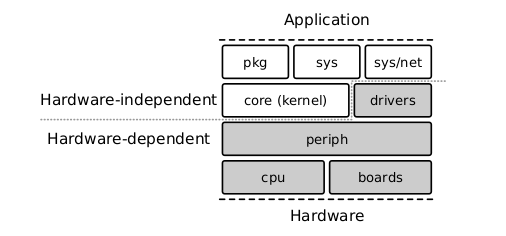
\includegraphics[width=0.8\linewidth]{riot_code}
    \caption{Structure elements of RIOT, see \cite[p.~3]{riot}}
    \label{fig:riot_code}
  \end{figure}

    Multi-threading is a builtin feature for RIOT to offer several benefits: (a) clear 
    logical separation between different tasks, (b) straightforward task prioritization, 
    and (c) easier integration of external code \cite[p.~4]{riot}. Various synchronization primitives, such
    as mutex, semaphore, and message passing (\textbf{msg}) are provided by RIOT kernel.
    Multi-threading can also be optional in the case of extremely low-memory usage of the application.

    RIOT's kernel employs a scheduler that uses fixed priorities and preemption with O(1) operations, 
    enabling soft real-time capabilities. Specifically, the time required to interrupt and switch 
    between threads is bounded by a small upper limit, as operations like context saving, selecting 
    the next thread, and context restoring are deterministic. The system follows a class-based 
    run-to-completion scheduling policy, where the highest-priority active thread is executed and 
    can only be interrupted by interrupt service routines (ISRs). This scheduler allows RIOT to 
    effectively prioritize tasks, ensuring that high-priority events can preempt lower-priority 
    tasks as needed.

    RIOT's scheduler operates in a tickless manner, meaning it does not rely on CPU time slices 
    or periodic system timer ticks. As a result, the system remains in a low-power state unless 
    an actual event occurs, such as an interrupt triggered by hardware. Wake-up events can be 
    initiated by a transceiver receiving a packet, timers expiring, buttons being pressed, or 
    similar activities. When no threads are in a running state and no interrupts are pending, 
    the system automatically switches to the idle thread, which has the lowest priority. 
    The idle thread, in turn, transitions the system into the most energy-efficient mode available 
    thereby reducing energy consumption.
\section{GNRC}
\subsection{Overview \& Architecture}
  The GNRC (short for generic) network stack is the default network stack for RIOT \cite{gnrc}. It was designed
  as a replacement for the previous monolithic and unmaintainable network stack of RIOT \cite{tcp}.
  The old stack was lack of unified interfaces, making it difficult to achieve modularity, testability,
  and extensibility. Furthermore, as most of the networks were using their own buffers, the memory
  footprint was increased, creating a need for significant data copying between layers, thus leading
  to a reduction in overall performance. These limitations drove the creation of the "gnrc" network stack 
  to replace the previous one.

  The design objectives of the generic network stack encompass a low memory footprint, full-featured
  protocols, modular architecture, support for multiple network interfaces, parallel data handling
  and customization during compilation time.

  \begin{figure}[h]
    \centering
    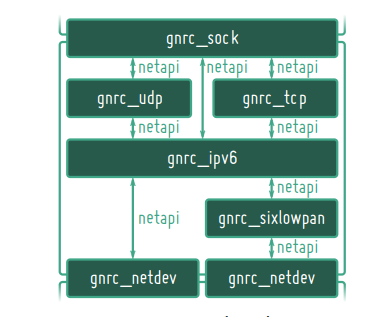
\includegraphics[width=0.5\linewidth]{netarch}
    \caption{GNRC Network Stack}
    \label{fig:netarch}
  \end{figure}

  Figure \ref{fig:netarch} illustrates the architecture of the GNRC network stack. Using multi-threading
  features and RIOT's thread-targeted IPC, every networking module runs in its own thread, communicating
  with other modules via the message queue. The messages passing between the network threads follow 
  a clearly defined format called ``\textit{netapi}'' in GNRC. A network registry called ``\textit{netreg}''
  is used for a network thread to search for a module that is interested in receiving the next packet, using
  the packet's type. Modules that want to receive certain types can register with this registry. While
  traversing through the stack, a packet is stored in the centralized GNRC packet buffer ``\textit{pktbuf}''.
  With this architecture, GNRC attains the required modularity and simplifies testing. 
  It also offers an easy way to prioritize different components of the stack, by assigning different 
  priorities to the threads running the protocols and allowing the operating system’s process 
  scheduler  to handle these priorities. The trade-off of this design is a performance penalty compared to
  straightforward function calls, as IPC involves context switches and context saves. However, this overhead
  is shown to be only one order of magnitude slower than a direct function call on real IoT hardware \cite[section 4.1]{oldwines}.

\subsection{The Packet Buffer - pktbuf}
  \begin{figure}[h]
    \centering
    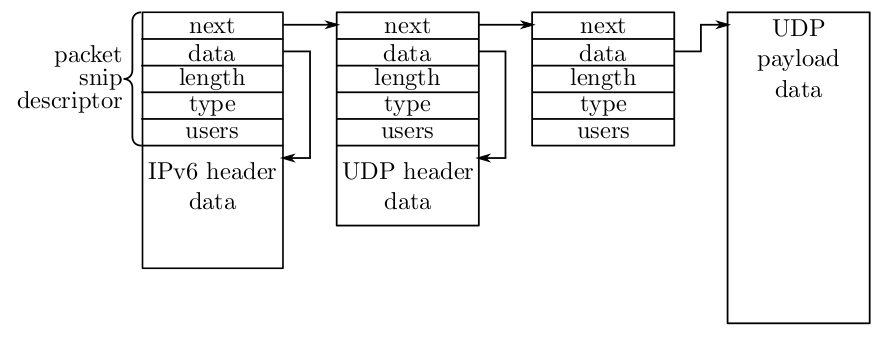
\includegraphics[width=\linewidth]{pktsnip}
    \caption{An example of a packet in transmission in the GNRC packet buffer, see \cite[p.~22]{gnrc}}
    \label{fig:pktsnip}
  \end{figure}

  Packets in GNRC are stored in a packet buffer called \textit{pktbuf}, consisting of variable-length 
  segments known as “packet snips” (see Figure \ref{fig:pktsnip}). These snips are typically used 
  to distinguish between different headers and payloads. The packet data, along with the structures 
  describing the packet snips, is stored in arrays allocated in static memory, although the API can 
  theoretically support dynamic allocation on the memory heap. Packet snips can be labeled with a 
  type to indicate the content of the packet. To create a packet snip in pktbuf, a user can 
  use the function \texttt{gnrc{\_}pktbuf{\_}add()}, which takes all user-controllable fields of a packet snip 
  (\texttt{next}, \texttt{data}, \texttt{length}, and \texttt{type}) as arguments and returns the new snip.

  With minimal packet duplication across the stack, data is being copied or moved as 
  infrequently as possible from the network interface to the application, ideally only once at each
  end-point of the stack and vice versa. This approach allows the structures that describe the packet 
  (referred to as the ``packet snip descriptor'' in Figure \ref{fig:pktsnip}) to be stored 
  independently of the actual data, enabling the marking of a packet header without requiring 
  to move data around.

  To ensure safety in concurrency, a reference counter (\texttt{user}) is maintained in a packet
  snip to keep track of the using threads. The APIs that handle the increment and the decrement of
  the counter are \texttt{gnrc{\_}pktbuf{\_}hold()} and \texttt{gnrc{\_}pktbuf{\_}release()}. The packet is
  removed from the packet buffer when the counter hits 0.

  When a thread starts to write to a packet and the reference counter is greater than one, the packet
  snip and all its next pointer will be cloned using a copy-on-write approach, resulting in the decrement 
  of the original snip's reference counter by one. For minimal duplication, the pointers reaching the
  current snip will be copied, creating a tree structure for the packet within the packet buffer, hence
  reversing the order of packet snips for a received packet. The packet snips now starts with the payload
  and end with the header of the lowest layer, whilst a packet in transmission retains the order 
  in which it will be sent, reducing the number of pointers needed for the tree structure. Nevertheless,
  it's crucial to note that data will be typically kept in the order it was received by the packets
  in reception. The only thing to be reversed is the packet descriptor list that marks the data.
  When a packet (i.e., the first snip in a packet snip list) is released by a thread, its own 
  snips will be removed from the packet buffer, with any of its copy snips still persist.
  The implementation of this feature is implemented in the \texttt{gnrc{\_}pktbuf{\_}start{\_}write()}
  function.

  This certain way of storing packets brings the merits of parallel data handling and low-memory
  footprint to GNRC, while avoiding duplication across the network stack.

\subsection{GNRC's Module Registry - netreg}
  The \textit{netreg} API provides a central directory to the generic network stack. When the
  thead of a network module is created, it also registered in \textit{netreg} using its thread
  PID and ``NETTYPE'' - the kind of information that it is interested in. For example, an IPv6
  module registers with its PID and type ``NETTYPE{\_}IPV6''. If the UDP module wants to dispatch
  the packet down the stack, \textit{netreg} would be used to search for threads registered
  with type ``NETTYPE{\_}IPV6''. Using \textit{netapi}, the module then send a pointer to the pktbuf-allocated
  packet to every interested thread.

\subsection{Network Interfaces}
  In GNRC, network interfaces run in their own threads and communicate with the network layer
  via \textit{netapi}. Within a network interface thread, MAC protocol are implemented
  and interact directy with network device drivers through the \textit{netdev} API. This direct
  access are required since some link-layer protocols, such as TDMA-based MAC, need minimal
  delay when acessing the device. To reduce the overhead of dealing with L2 headers, the header
  formats of each network interface's L2 protocol are converted into netif \textit{netif} header -
  a general interface header format. Source and destination L2 addresses, header's length, along side
  with additional link metrics utilized for routing protocol, such LQI and RSSI are included is this
  \textit{netif} header. A unified conversion API for popular L2 protocols ensures that 
  no redundant porting efforts are necessary.
